\documentclass{beamer}
\usepackage{../tut-slides}
\usepackage{../mathoperatorsAuD}

\usepackage{lmodern}
\usepackage{amsmath,amssymb}
\usepackage{wasysym}
\usepackage{stmaryrd}
\usepackage{enumerate}
%\usepackage[inline]{enumitem} 		%customize label
%\newcommand{\labelitemi}{\raisebox{1pt}{\scalebox{.9}{$\blacktriangleright$}}}
%\newcommand{\labelitemii}{$\vartriangleright$}
%\newcommand{\labelitemiii}{--}
\setbeamertemplate{itemize item}{\raisebox{1pt}{\scalebox{.9}{$\blacktriangleright$}}}
\setbeamertemplate{itemize subitem}{$\vartriangleright$}

\usepackage{booktabs}
\usepackage{tabularx}
\usepackage{tabu}
\newcommand*\head{\rowfont{\bfseries}}
\newcommand*{\tw}{\rowfont{\ttfamily}}
\renewcommand{\tabularxcolumn}[1]{>{\hspace{0pt}}m{#1}}
\usepackage{multirow}

\usepackage{cancel}

\usepackage{empheq}
\newcommand*\widefbox[1]{\fbox{\hspace{2em} #1 \hspace{2em}}}

\usepackage{tcolorbox}
\newtcolorbox{mymathbox}[1][]{colback=white, sharp corners, #1}

\usepackage{xcolor}
\usepackage{listings}
\lstset{numbers=left, 
	numberstyle=\tiny, 
	breaklines=true,
	backgroundcolor=\color{cdgray!20},
	numbersep=5pt,
	language=C,
	tabsize=2,
	basicstyle=\footnotesize\ttfamily,
	showstringspaces=false} 

\DeclareMathOperator{\ack}{\mathbf{ack}}
\usepackage{MnSymbol}

\newcommand{\col}[1]{\textcolor{cdpurple}{#1}}
\newcolumntype{R}[1]{>{\centering\arraybackslash}p{#1}}
\usepackage{tabularx}
\renewcommand{\tabularxcolumn}[1]{m{#1}}

\usepackage{qtree}

\begin{document}	
	\title{Algorithmen und Datenstrukturen}
	\subtitle{Übung 9: Sortieren, Suchen \& Korrigieren}
	\author{Eric Kunze}
	\email{eric.kunze@mailbox.tu-dresden.de}
	\city{TU Dresden}
%	\institute{Lehrstuhl für Grundlagen der Programmierung}
	\titlegraphic{
\includegraphics[width=2cm]{../TUD-white.pdf}}
	\date{19.12.2019}

	\maketitle


%%%%%%%%%%%%%%%%%%%%%%%%%%%%%%%%%%%%%%%%%%%%%%%%%%%%%%%%%%%%%%%%%%%%%%%%%%%%%

\begin{frame} \frametitle{Darum geht's heute}
	\centering
	
	{\LARGE \texttt{void (*(*f[])())()}} \\
	\vspace{2em}
	
	\begin{ttfamily}
		\begin{tabular}{ll}
			f              & -- f \\
			f[]            & -- is an array \\
			*f[]           & -- of pointers  ([] has higher precedence than *) \\
			(*f[])()       & -- to functions \\
			*(*f[])()      & -- returning pointers \\
			(*(*f[])())()  & -- to functions \\
			void (*(*f[])())(); & -- returning void \\
		\end{tabular}
	\end{ttfamily}

	\pause
	\vspace{3em}
	{\LARGE \textbf{\dots NICHT} \smiley
}\end{frame}
\begin{frame} \frametitle{Quicksort}
	\centering
	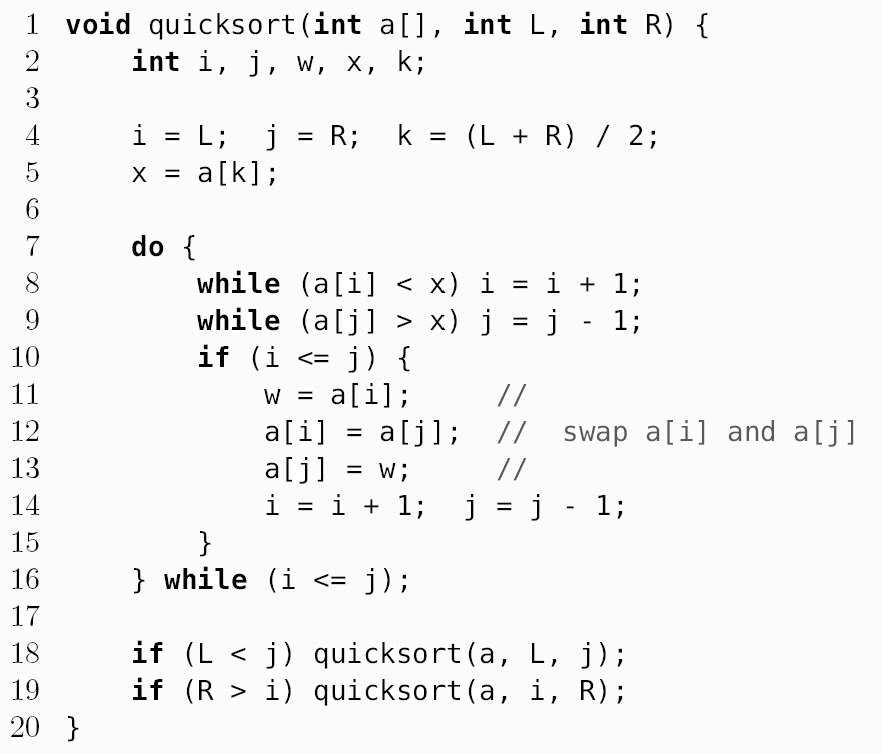
\includegraphics[height=.95\textheight]{./tut09_quicksort.jpg}
\end{frame}

\begin{frame} \frametitle{Aufgabe 1}
	\begin{columns}[t]
		\begin{column}{\dimexpr0.5\linewidth-\fboxrule-\fboxsep}
			\textbf{1. Durchlauf} \\[1em]
			\centering
			
			\begin{tabular}{ccccc}
				9 & 13 & \fbox{7} & 6 & 10 \\
				$\uparrow$ & & & & $\uparrow$ \\
				$i$ &&&& $j$ \\
				
				9 & 13 & \fbox{7} & 6 & 10 \\
				$\uparrow$  &&& $\uparrow$ &\\
				$i$ &&& $j$ & \\
				
				6 & 13 & \fbox{7} & 9 & 10 \\
				& $\uparrow$ & $\uparrow$ &&\\
				& $i$ & $j$ & & \\
				
				6 & \fbox{7} & 13 & 9 & 10 \\
				& $\uparrow$  & $\uparrow$ &&\\
				& $j$ & $i$ && \\
			\end{tabular}
		\end{column}
		\begin{column}{\dimexpr0.5\linewidth-\fboxrule-\fboxsep}
			\textbf{2. Durchlauf} \\[1em]
			\centering
			
			\begin{tabular}{ccc||ccc}
				&\fbox{6} & 7 & 13 & \fbox{9} & 10 \\
				&$\uparrow$ & $\uparrow$ & $\uparrow$ && $\uparrow$ \\
				&$i$ & $j$ & $i$ && $j$ \\
				
				&\fbox{6} & 7 & 13 & \fbox{9} & 10 \\
				&$\uparrow$ & & $\uparrow$ & $\uparrow$ & \\
				&$i,j$ & & $i$ & $j$ & \\
				
				&\fbox{6} & 7 & \fbox{9} & 13 & 10 \\
				$\uparrow$ & & $\uparrow$ & $\uparrow$ & $\uparrow$ & \\
				$j$ & & $i$ & $j$ & $i$ & \\
			\end{tabular}
		\end{column}
	\end{columns}
\end{frame}

\begin{frame} \frametitle{Aufgabe 1}
	\centering
	\textbf{3. Durchlauf} \\[1em]
	
	\begin{tabular}{cc||cc||cc}
		6 & 7 & 9 & & \fbox{13} & 10 \\
		& & & & $\uparrow$ & $\uparrow$ \\
		& & & & $i$ & $j$ \\
		
		6 & 7 & 9 & & 10 & \fbox{13} \\
		& & & $\uparrow$ & & $\uparrow$ \\
		& & & & $j$ & $i$ \\
	\end{tabular}
	\vspace{1cm}
	
	\textbf{Ergebnis:} \\
	\texttt{[6,7,9,10,13]}
\end{frame}

%%%%%%%%%%%%%%%%%%%%%%%%%%%%%%%%%%%%%%%%%%%%%%%%%%%%%%%%%%%%%%%%%%%%%%%%%%%%%%%%%%%

\begin{frame} \frametitle{Heapsort}
	\begin{itemize}
		\item Bäume sind nur Veranschaulichung
		\item Algorithmus arbeitet auf Listen
		\item zwei Phasen
		\begin{itemize}
			\item \textbf{1. Phase:} Einsortieren in den Heap und Herstellen der Heap-Eigenschaft
			\item \textbf{2. Phase:} Führe Sortierschritt wiederholt durch:
			\begin{itemize}
				\item Tausch von Wurzel und ''letztem`` Element (tiefste Ebene, ganz rechts)
				\item Fixiere dieses Element
				\item Sinkenlassen des neuen Wurzelelements
			\end{itemize}
		\end{itemize}
	\end{itemize}
\end{frame}

\begin{frame} \frametitle{Aufgabe 2 --- Phase 1}
	\begin{tabularx}{\linewidth}{m{.8cm} m{4cm}m{.8cm}m{4cm}}
		& \onslide+<1->{\Tree [ .2 [ .4 [ .9  [ .8 ] [ .5 ]] [ .13 [ .18 ]  ] ] [ .17 [ .20 ] [ .12 ] ] ]}
		&
		\onslide+<2->{$\overset{s(13), \ s(9)}{\longrightarrow}$}
		&
		\onslide+<3->{\Tree [ .2 [ .4 [ .9  [ .8 ] [ .5 ]] [ .18 [ .13 ]  ] ] [ .17 [ .20 ] [ .12 ] ] ]} \\
		\onslide+<4->{$\overset{s(4), s(17)}{\longrightarrow}$}
		&
		\onslide+<5->{\Tree [ .2 [ .18 [ .9  [ .8 ] [ .5 ]] [ .13 [ .4 ]  ] ] [ .20 [ .17 ] [ .12 ] ] ]}
		&
		\onslide+<6->{$\overset{s(2)}{\longrightarrow}$}
		&
		\onslide+<7->{\Tree [ .20 [ .18 [ .9  [ .8 ] [ .5 ]] [ .13 [ .4 ]  ] ] [ .17 [ .2 ] [ .12 ] ] ]}
	\end{tabularx}
\end{frame}

\begin{frame} \frametitle{Aufgabe 2 --- Phase 2}
	\begin{tabularx}{\linewidth}{m{.8cm}m{4cm}m{.8cm}m{4cm}}
		\onslide+<1->{$\overset{\text{Tausch}}{\longrightarrow}$}
		&
		\onslide+<2->{\Tree [ .4 [ .18 [ .9  [ .8 ] [ .5 ]] [ .13 [ .\fbox{20} ]  ] ] [ .17 [ .2 ] [ .12 ] ] ]}
		&
		\onslide+<3->{$\overset{s(4)}{\longrightarrow}$}
		&
		\onslide+<4->{\Tree [ .18 [ .13 [ .9  [ .8 ] [ .5 ]] [ .4 [ .\fbox{20} ]  ] ] [ .17 [ .2 ] [ .12 ] ] ]} \\
		\onslide+<5->{$\overset{\text{Tausch}}{\longrightarrow}$ }
		&
		\onslide+<6->{\Tree [ .5 [ .13 [ .9  [ .8 ] [ .\fbox{18} ]] [ .4 [ .\fbox{20} ]  ] ] [ .17 [ .2 ] [ .12 ] ] ]} 
		&
		\onslide+<7->{$\overset{s(5)}{\longrightarrow}$}
		&
		\onslide+<8->{\Tree [ .17 [ .13 [ .9  [ .8 ] [ .\fbox{18} ]] [ .4 [ .\fbox{20} ]  ] ] [ .12 [ .2 ] [ .5 ] ] ]}  \\
	\end{tabularx}
\end{frame}


%%%%%%%%%%%%%%%%%%%%%%%%%%%%%%%%%%%%%%%%%%%%%%%%%%%%%%%%%%%%%%%%%%%%%%%%%%%%%%%%%%%


\begin{frame} \frametitle{KMP-Algorithmus}
	\begin{itemize}
		\item Mustersuche in (großen) Texten
		\item Ziel: Verschiebung des Musters um mehr als eine Position bei Nichtübereinstimmung.
		\item Methode: Ermittlung einer Verschiebetabelle {\large $\texttt{Tab[]}$}
		\item Bedeutung des Eintrags {\large $\texttt{Tab[i]=j}$}: \\
		Bei Nichtübereinstimmung an Stelle $i$ wird Position $j$ des Musters an aktueller Vergleichsstelle angelegt.
	\end{itemize}
\end{frame}

\begin{frame} \frametitle{KMP-Algorithmus}
	\small
	Suche das Muster \texttt{aaabaaaa} im Text \texttt{aaabaaabaaacaaabaaaa}.
	\begin{center}
		\begin{tabular}{l|cccccccc}
			Position &  0 &  1 &  2 &  3 &  4 &  5 &  6 &  7 \\ \hline
			Pattern  &  a &  a &  a &  b &  a &  a &  a &  a \\ \hline
			Tabelle  & -1 & -1 & -1 &  2 & -1 & -1 & -1 &  3 \\
		\end{tabular}
	\end{center}

	\renewcommand*{\arraystretch}{.7}
	\setlength{\tabcolsep}{1pt}
	
	Erster Versuch:
	\begin{center}
		\begin{tabular}{ccccccccccccccccccccc}
			a & a & a & b & a & a & a & \textbf{b} & a & a & a & c & a & a & a & b & a & a & a & a \\
			a & a & a & b & a & a & a & \textbf{a}
		\end{tabular}
	\end{center}
	Tabelleneintrag an Position $7$ ist $3$, d.h. $\texttt{Tab[7] = 3}$ --- Lege Position $3$ des Musters an aktueller Vergleichsposition an:
	\begin{center}
		\begin{tabular}{ccccccccccccccccccccc}
			a & a & a & b & a & a & a & b & a & a & a & \textbf{c} & a & a & a & b & a & a & a & a \\
			&   &   &   & a & a & a & b & a & a & a & \textbf{a}
		\end{tabular}
	\end{center}
	Erneute Verschiebung liefert schließlich:
	\begin{center}
		\begin{tabular}{ccccccccccccccccccccc}
			a & a & a & b & a & a & a & b & a & a & a & c & a & a & a & b & a & a & a & a \\
			&   &   &   &   &   &   &   &   &   &   &   & a & a & a & b & a & a & a & a &
		\end{tabular}
	\end{center}
\end{frame}


\begin{frame} \frametitle{KMP-Algorithmus --- Die Zyklenmethode}
	Zwei Phasen:
	\pause
	\begin{itemize}
		\item \textbf{1. Phase:} Markieren der längsten Teilwörter im Pattern, die mit einem Präfix übereinstimmen
		\begin{itemize}
			\item ein Zyklus beginnt an einer Patternposition $\texttt{i}$ falls $\texttt{i} \neq \texttt{0}$ und $\texttt{Pat[0] = Pat[i]}$
			\item ein Zyklus endet an der kleisten Patternposition $\texttt{i+m}$, sodass $\texttt{Pat[m+1]} \neq \texttt{Pat[i+m+1]}$
		\end{itemize}
	\pause
	\item \textbf{2. Phase:} Bestimmung der Tabelleneinträge
	\begin{itemize}
		\item $\texttt{Tab[0] = -1}$
		\item Tabelleneinträge nach einem Zyklus: \\
		\textit{Länge des längsten dort endenden Zyklus}
		\item Tabelleneinträgen in einem Zyklus: \\
		\textit{Tabelleneintrag der derzeitigen Position im längsten laufenden Zyklus}
		\item verbleibende Einträge: \texttt{0}
	\end{itemize}
	\end{itemize}
\end{frame}
\begin{frame} \frametitle{Aufgabe 3}
	\textbf{Teil (a)} \hspace{3em}
	Pattern: {\large \texttt{aabaaacaab}} \\[1em]
	\pause
	
	\begin{center}
		\begin{tabular}{l|cccccccccc}
			Position &  0 &  1 &  2 &  3 &  4 &  5 &  6 &  7 &  8 &  9 \\ \hline
			Pattern  &  a &  a &  b &  a &  a &  a &  c &  a &  a &  b \\ \hline
			Tabelle  & -1 & -1 &  1 & -1 & -1 &  2 &  2 & -1 & -1 &  1 \\
		\end{tabular}
	\end{center}
	
	\pause

	\textbf{Teil (b)}
	\begin{center}
		\begin{tabular}{l|cccccc}
			Position &  0 &  1 &  2 &  3 &  4 &  5 \\ \hline
			Pattern  &  \textit{c} &  \textit{b} &  c &  c &  b &  \textit{a} \\ \hline
			Tabelle  & -1 &  0 & -1 &  1 &  0 &  2 \\
		\end{tabular}
	\end{center}
	
\end{frame}

%%%%%%%%%%%%%%%%%%%%%%%%%%%%%%%%%%%%%%%%%%%%%%%%%%%%%%%%%%%%%%%%%%%%%%%%%%%%%%%%%%%


\begin{frame} \frametitle{Levenshtein-Distanz}
	\textbf{Kosten} zur Überführung eines Wortes $w = w_1 \dots w_n$ in ein Wort $v = v_1 \dots v_k$ ; schreibe $d(w_1 \dots w_j, v_1 \dots v_i) = d(j,i)$.
	\begin{align*}
		d(0,i) &= i \\
		d(j,0) &= j \\
		d(j,i) &= \min \menge{ d(j,i-1) + 1, d(j-1,i) + 1 , d(j-1, i-1) + \delta_{j,i}}
	\end{align*}
	für alle $1 \le j \le n$ und alle $1 \le i \le k$ wobei
	\begin{equation*}
		\delta_{j,i} = \begin{cases}
		1 & \text{wenn } w_j \neq v_i \\
		0 & \text{sonst}
		\end{cases} 
	\end{equation*}
	\pause
	\textbf{Anschaulich:} 
	Überlagerung durch Pattern
	$\to$ Pfeile zeigen ''Ursprung`` des Minimums an
	\begin{equation*}
		w_j \neq v_i : \quad \begin{array}{|c|c|}
			\hline +1 & +1 \\ \hline +1 & ? \\ \hline
		\end{array}
		\qquad \qquad
		w_j = v_i : \quad 
		\begin{array}{|c|c|}
		\hline +0 & +1 \\ \hline +1 & ? \\ \hline
		\end{array}
	\end{equation*}

\end{frame}
\begin{frame} \frametitle{Aufgabe 4}
		\centering
		\renewcommand*{\arraystretch}{.7}
		\setlength{\tabcolsep}{3pt}
			\begin{tabular}{l|ccccccccccccccc}
				$d(j,i)$ &       &       & \textbf{D} &       & \textbf{i} &       & \textbf{s} &       & \textbf{t} &       & \textbf{a} &       & \textbf{n} &       & \textbf{z} \\ \hline \\
				& 0     & $\rightarrow$ & 1     & $\rightarrow$ & 2     & $\rightarrow$ & 3     & $\rightarrow$ & 4     & $\rightarrow$ & 5     & $\rightarrow$ & 6     & $\rightarrow$ & 7 \\
				& $\downarrow$ & $\searrow$ &       &       &       &       &       &       &       &       &       &       &       &       &  \\
				\textbf{D}     & 1     &       & 0     & $\rightarrow$ & 1     & $\rightarrow$ & 2     & $\rightarrow$ & 3     & $\rightarrow$ & 4     & $\rightarrow$ & 5     & $\rightarrow$ & 6 \\
				& $\downarrow$ &       & $\downarrow$ & $\searrow$ &       &       &       &       &       &       &       &       &       &       &  \\
				\textbf{i}     & 2     &       & 1     &       & 0     & $\rightarrow$ & 1     & $\rightarrow$ & 2     & $\rightarrow$ & 3     & $\rightarrow$ & 4     & $\rightarrow$ & 5 \\
				& $\downarrow$ &       & $\downarrow$ &       & $\downarrow$ & $\searrow$ &       & $\searrow$ &       & $\searrow$ &       & $\searrow$ &       &       &  \\
				\textbf{n}     & 3     &       & 2     &       & 1     &       & 1     & $\rightarrow$ & 2     & $\rightarrow$ & 3     &       & 3     & $\rightarrow$ & 4 \\
				& $\downarrow$ &       & $\downarrow$ &       & $\downarrow$ & $\searrow$ &       & $\searrow$ &       & $\searrow$ &       & $\searrow$ & $\downarrow$ & $\searrow$ &  \\
				\textbf{s}     & 4     &       & 3     &       & 2     &       & 1     & $\rightarrow$ & 2     & $\rightarrow$ & 3     & $\rightarrow$ & 4     &       & 4 \\
				& $\downarrow$ &       & $\downarrow$ &       & $\downarrow$ &       & $\downarrow$ & $\searrow$ &       &       &       &       &       &       &  \\
				\textbf{t}     & 5     &       & 4     &       & 3     &       & 2     &       & 1     & $\rightarrow$ & 2     & $\rightarrow$ & 3     & $\rightarrow$ & 4 \\
				& $\downarrow$ &       & $\downarrow$ &       & $\downarrow$ &       & $\downarrow$ &       & $\downarrow$ & $\searrow$ &       &       &       &       &  \\
				\textbf{a}     & 6     &       & 5     &       & 4     &       & 3     &       & 2     &       & 1     & $\rightarrow$ & 2     & $\rightarrow$ & 3 \\
				& $\downarrow$ &       & $\downarrow$ &       & $\downarrow$ & $\searrow$ & $\downarrow$ &       & $\downarrow$ &       & $\downarrow$ & $\searrow$ &       & $\searrow$ &  \\
				\textbf{s}     & 7     &       & 6     &       & 5     &       & 4     &       & 3     &       & 2     &       & 2     & $\rightarrow$ & 3 \\
			\end{tabular}
\end{frame}

\begin{frame} \frametitle{Aufgabe 4}
	Alignments mit minimaler Levenshtein-Distanz:
	
	\centering
	
	\begin{tabular}{cccccccc}
		D & i & n & s & t & a & $\ast$ & s \\
		$|$ & $|$ & $|$ & $|$ & $|$ & $|$ & $|$ & $|$ \\
		D & i & $\ast$ & s & t & a & n & z \\
		  &   & \textit{d} &   &   &   & \textit{i} & \textit{s} \\
	\end{tabular}

	\vspace{3em}
	
	\begin{tabular}{cccccccc}
		D & i & n & s & t & a & s & $\ast$ \\
		$|$ & $|$ & $|$ & $|$ & $|$ & $|$ & $|$ & $|$ \\
		D & i & $\ast$ & s & t & a & n & z \\
		&   & \textit{d} &   &   &   & \textit{s} & \textit{i} \\
	\end{tabular}
\end{frame}



%%%%%%%%%%%%%%%%%%%%%%%%%%%%%%%%%%%%%%%%%%%%%%%%%%%%%%%%%%%%%%%%%%%%%%%%%%%%%%%%%%%

\end{document}
